\newcommand{\tcr}{\textcolor{red}}
\FloatBarrier
\subsubsection{Quantum noise reduction with squeezed states of light}\label{subsec:QNRsqz}
%\emph{Author(s): \textbf{Andre Thuering}, Helge Mueller-Ebhardt, Keiko Kokeyama, Sergey Tarabrin \\}
The following description of squeezed light usage in gravitational wave detectors is an excerpt of the article \cite{SqueezingSchnabel2010}. 
At first glance, quantum physics imposes a fundamental limit on metrology---the science of measurement---and thus imposes a corresponding limit on the sensitivity of GW detectors.  A fundamental problem in optical interferometry is
the random distribution of photons arriving at the photodiodes.  This statistical fluctuations obscure the tiny power variations caused by GW signals. Fortunately, quantum physics also provides a solution to this problem via the concept of quantum entanglement.

\longetbox{h}{box:quantummetrology}{Quantum metrology with squeezed states of light}{%
``Quantum metrology'' uses quantum entanglement to improve the measurement precision beyond the limit set by measurement counting noise. The first such proposal was made by C.M.\ Caves in 1981~\cite{Caves1981}.
He showed that the quantum noise limited sensitivity  in a shot noise dominated interferometer can be enhanced by the injection of a broadband (frequency independent) squeezed field  into the interferometers signal port.  Furthermore he stated that ``[\ldots]the greatest potential usefulness of squeezed states lies in its ability to increase the sensitivity without increasing the circulating laser light power[\ldots]''. Accordingly at a point, where the interferometer performance will be limited by the available laser power or thermal load in its optics, squeezed light injection can be used to either relax the high power requirement or to increase the sensitivity further. Fig.~\ref{fig:SqzIll} illustrates the principle of squeezed light enhanced metrology.
\begin{figure}[H]
  \centering
  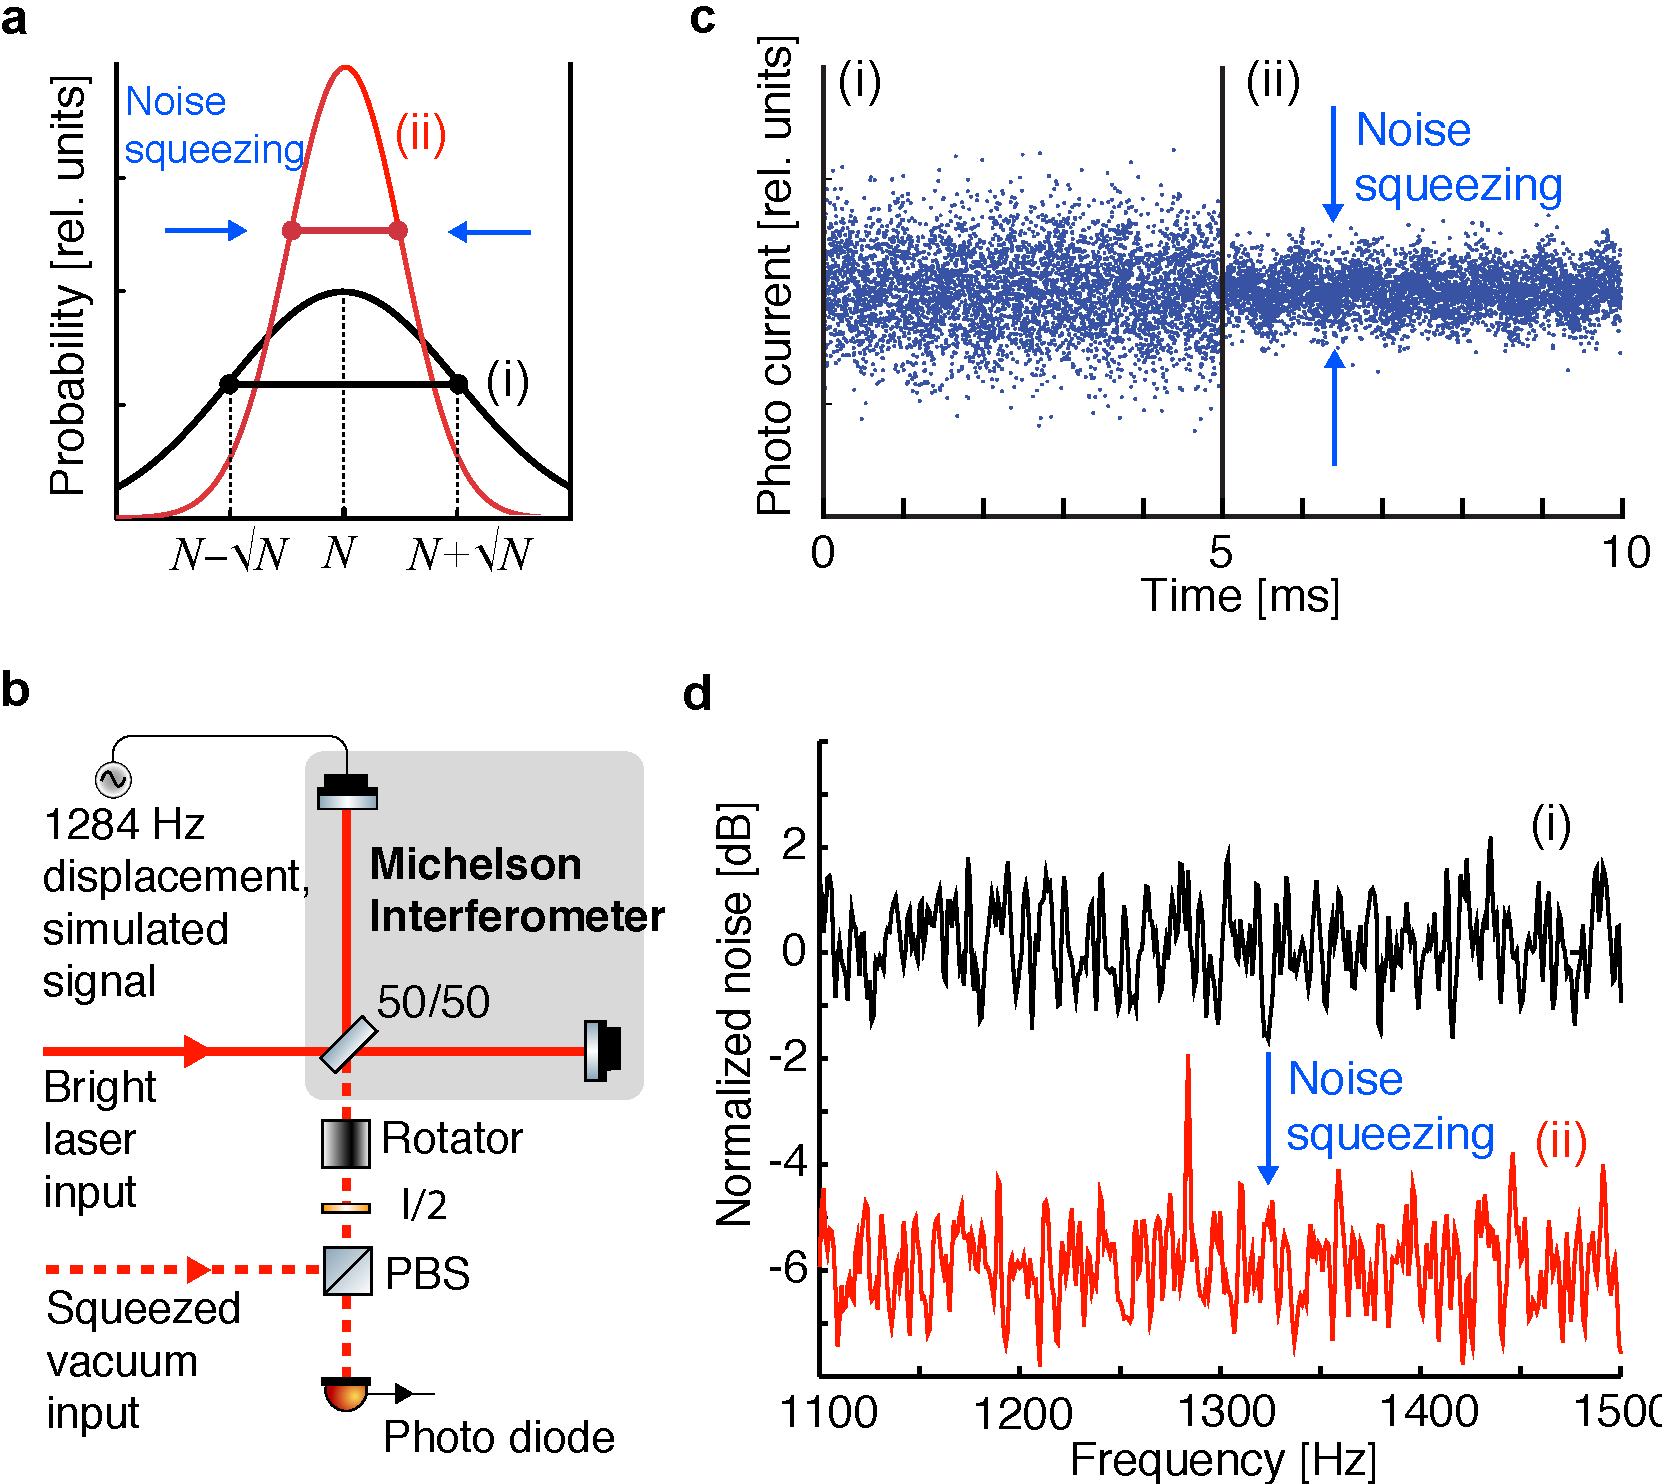
\includegraphics[scale=0.42]{./Sec_Optics/SqzIllustration.pdf}
\caption[Squeezed light enhanced metrology]{{\textbf{Squeezed light enhanced metrology} \; (a) For large photon numbers $N$, squeezed light shows a photon counting statistic with a standard deviation smaller than $\pm \sqrt{N}$. In all panels, (i) correspond to shot-noise and (ii) to 6\,dB squeezed noise. (b) A squeezed vacuum beam is injected into the dark signal port of a Michelson interferometer, in addition to the conventional bright laser input. The squeezed beam leads to path entanglement of the light fields in the two arms and to an improved signal to noise ratio, as shown on the right. Without squeezing, the optical path length modulation at 1284\,Hz is neither visible in the time series of the photo-electron current (c, simulation by B. Hage, AEI) nor in its noise power spectrum (d, measurement, courtesy of H. Vahlbruch, AEI \cite{VahlbruchPhD08}). In (c) as well as in (d), the signal is clearly visible when squeezing is applied (ii).}
}\label{fig:SqzIll}
\end{figure}%
}



Squeezed states \cite{Yuen1976,Walls1983,Breitenbach1997,Dodonov2002} belong to the class of so-called \textit{nonclassical} states of light.
Generally, nonclassical states are those that cannot be described by a classical (positive valued) probability distribution using the coherent states as a basis (the $P$-representation) \cite{GerryKnight}. Let us first consider the coherent states. If light in a coherent state is absorbed by a photodiode, mutually independent photon `clicks' (in terms of photo-electrons) are recorded, a process that is described by Poissonian counting statistics. Due to quantum mechanics, every individual `click' is not predictable, but rather the result of a truly random process. If the number of photons per time interval is large ($N\!>\!\!>\!1$), its standard deviation is given by $\sqrt{N}$, see Fig.~\ref{fig:SqzIll}\,a\,(i). This uncertainty gives rise to \textit{shot-noise}. For a \emph{squeezed} light beam, the detection of photons is not time-independent but instead contains quantum correlations.  Nevertheless, the photon statistics still cannot be predicted by some external clock. It instead shows auto-correlations that give rise to a reduced standard deviation, as shown in Fig.~\ref{fig:SqzIll}\,a\,(ii). The correlations might be described in the following way. Whenever the quantum statistics might drive the actual photon number above the average value $N$, a similar number of photons destructively interfere with the main body of photons providing a (partial) compensation of the fluctuation. These quantum correlations \textit{squeeze} the interferometer's shot-noise below its natural value. Another complementary way of describing the properties of squeezed states is based on the phase space quasi-probability distribution using the amplitude and phase quadratures of a light wave (the Wigner function) \cite{Walls1983,GerryKnight}.

A squeezed state that contains only quantum-correlated photons with no coherent amplitude is called a \textit{squeezed vacuum state} \cite{GerryKnight}. If such a state is overlapped with a coherent laser beam on a semi-transparent beam splitter, two beam splitter outputs are generated which are quantum correlated. As a consequence, the overall (bi-partite) quantum state cannot be written in terms of products of the two beam splitter output states. Such a quantum state is called non-separable or \textit{entangled}. This is exactly what happens if a squeezed state is injected into the signal output port of a laser interferometer for GW detection (Fig.~\ref{fig:SqzIll}\,b). The two \textit{high-power} light fields in the interferometer arms get entangled and the light's quantum fluctuations in the two arms are correlated with each other. Although the fluctuations are not predictable from the outside, they provide an improved signal-to-noise ratio in the interferometer. Recall that an interferometer measures the optical path length change in one interferometer arm with respect to the other arm. If the quantum noise in the two arms is correlated it will cancel out.
This entanglement interpretation was not discussed in the initial proposal by Caves.  Nevertheless, it shows that the application of squeezed states in interferometers is a real application of quantum metrology by its very own definition. The entanglement produced by splitting a squeezed state at a semi-transparent beam splitter was tomographically characterized and quantified in \cite{DiGuglielmo2007}. Fig.~\ref{fig:SqzIll}\,c shows a simulated signal from a photodiode, without (i) and with (ii) \textit{squeezing}. The tiny modulation in the interferometer's output light due to the (simulated) passing GW is visible only with the improved signal-to-noise ratio. Fig.~\ref{fig:SqzIll}\,d shows the analogue in frequency space, i.e.\ after a Fourier transform of the photo current was applied.

The above paragraph shows that squeezed states can be conveniently combined with the extremely
high photon numbers of coherent light to improve a laser interferometer, as proposed in \cite{Caves1981}
and shown in Fig.~\ref{fig:SqzIll}\,b. In fact, the stronger the squeezing
factor \cite{Walls1983,GerryKnight} the greater the path entanglement and the signal-to-noise
improvement. %Very strong path entanglement is present in interferometers using so-called NOON-states instead of squeezed states.  NOON states are another class of nonclassical states \cite{GerryKnight04,HBu93,WPAUGZ04,AAS10}.   Unfortunately, the strong entanglement of a NOON state is extremely fragile, in particular if $N$ is large. Very recently a NOON-state with $N=5$ photons was demonstrated \cite{AAS10}. However, gravitational wave detectors use coherent high-power laser light with $N \approx 10^{23}$ photons per second. An improvement by use of NOON states is, therefore, far out of reach.

%\textcolor{red}{Overlap with Sec.~\ref{subsec:qnft}}.

Shortly after Caves proposed squeezed states of light for laser
interferometers in 1981, the first experimental demonstration of squeezed
light \cite{Slusher1985} and proof of principle demonstrations of
quantum metrology were achieved \cite{Xiao1987,Grangier1987}. In parallel, it was theoretically discovered that squeezed states offer even more advances in metrology than `just' reducing the quantum shot-noise.
From the early days of quantum physics, when fundamental
aspects of the measurement process were discussed, it was clear that,
in general, a measurement disturbs the system to be measured
\cite{Braginsky1999}. %Braginsky95}.
 The measurement of quantity $A$ (say
a position of a mirror) increases the uncertainty of the
non-commuting quantity $B$ (say the mirror's momentum). Both
observables are linked by a Heisenberg Uncertainty relation. For
repeated measurements of $A$, the increased uncertainty in $B$
disturbs the measurement of $A$ at later times. This is referred to
as \textit{quantum back-action noise}. Here, the back-action arises
from the fluctuating radiation pressure due to the reflected light \cite{CavesPRL451980}.
It is significant if the mirror's mass is low and a
large photon number is reflected. In the 1970s, ideas were developed
that showed how, in principle, back-action noise for continuous
measurements can be avoided. Such schemes were called
quantum-non-demolition (QND) measurements \cite{Thorne1978, BraginskyRMP1996}.
However, for laser interferometric GW detectors
using \textit{quasi-free} falling mirrors it remained unclear if QND schemes
exist. In \cite{CavesPRL451980,Caves1981} it was concluded that back-action noise
of a free mass position measurement can in principle not be avoided and, together with photon counting noise, defines a \textsl{standard
quantum limit} (SQL). In \cite{Yuen1983,Unruh1983} it was argued, however, that measurements below the
SQL of a free mass are indeed possible. The discussion
remained controversial \cite{CavesPRL1985} until Jaekel and Reynaud
\cite{Jaekel1990} were able to convincingly show that the cleverly
arranged squeezed states in a GW detector can simultaneously reduce
the shot-noise and the radiation pressure noise, by almost arbitrary
amounts (as long as most of the photons belong to the light's coherent displacement).
%\textcolor{red}{Refer to Sec.~\ref{subsec:qnft}, great overlap, arrange Secs properly... }

So far no experiment has achieved a position measurement with
sensitivity even at, let alone below, its standard quantum limit.
Eventually this will be achieved, possibly first in future
gravitational wave detectors.  Advanced detectors are in
fact designed to have a sensitivity at or just below their SQLs.
Once the SQL is reached, a new level of quantum metrology is achieved, because the position-momentum
uncertainty of the mirror becomes correlated with the quadrature
uncertainty of the reflected optical field. In this way, entanglement
between the mechanical and the optical system can be observed
\cite{Vitali2007}. This is all the more remarkable from the perspective of GW detectors
since we are talking about mirrors with masses of 40 kg, planned for
the upcoming Advanced LIGO \cite{aLIGO}, and even in the order of a 100\,kg concerning the envisaged LF-detector of ET.
Eventually, even two such mirrors might be projected via entanglement swapping
\cite{Pirandola2006} into an entangled state \cite{M-Ebhardt2008}.
Obviously quantum metrology opens the possibility for further
studies of the peculiarities of quantum physics at a macroscopic scale.



\FloatBarrier
\paragraph{Squeezed light for Gravitational wave astronomy}\label{subsec:SQZforGWD}
Laser interferometers for GW astronomy are facing extreme sensitivity requirements that can only be achieved if all available
tools, inclusive of quantum metrology, are combined in an elaborate measurement device.  Squeezed light must be generated in a non-linear
interaction. Squeezed light was first produced in 1985 by
Slusher et al.\ using four-wave-mixing in Na atoms in an optical
cavity \cite{Slusher1985}. Shortly after, squeezed light was also
generated by four-wave-mixing in an optical fibre \cite{Shelby1986}
and by parametric down-conversion in an optical cavity containing a
second order non-linear material \cite{Wu1986}. In these early day
experiments, squeezing of a few percent to 2  to 3\,dB were routinely observed (For an
overview of earlier experiments and squeezed light generation in
the continuous-wave as well as pulsed regime please refer to Ref.~\cite{BachorRalph2004}).


\begin{figure}[ht]
  \centering
  \includegraphics[scale = .41]{./Sec_Optics/SqzGen.pdf}
  \vspace{-1mm}
\caption{{\textbf{Generation of squeezed light} (a) A continuous-wave laser beam at the GW detector wavelength is first spatially filtered and then up-converted to a field at half the wavelength (second harmonic generation, SHG). That beam is then mode-matched into the `squeezing resonator' in which a tiny fraction of the up-converted photons are spontaneously down-converted by optical parametric amplification (OPA) producing a squeezed vacuum state. The squeezing factor is validated by a balanced homodyne detector (BHD). SHG as well as OPA are realized by a non-linear crystal (b), here a 6\,mm long MgO:LiNbO$_3$ crystal, inside an optical resonator (c) formed by an external cavity mirror and the dielectrically coated crystal back surface. The two non-linear resonators may be constructed in an identical way and are put into temperature stabilized housings (d).}
}
\label{fig:SqzGen}
\end{figure}

GW detectors are operated with high-power, quasi-monochromatic
continuous-wave laser light with an almost Fourier-limited spatial
distribution of a Gaussian TEM$_{00}$ mode. For a non-classical
sensitivity improvement, squeezed light in exactly the same
spatio-temporal mode must be generated and mode-matched into the
output port of the interferometer \cite{Caves1981}, providing
interference with the high-power coherent laser beam at the
interferometer's central beam splitter. High-power lasers for GW
astronomy are based on optically pumped solid-state crystals in
resonators \cite{Frede2006}%\textcolor{red}{refer to sec 'Pre-stabilized laser'}
, suggestive of a similar configuration for
a ``squeezed light resonator''. Fig.~\ref{fig:SqzGen}\,(a) shows a
schematic setup for generation of squeezed light that is built upon one of the very first squeezing experiments \cite{Wu1986}, a setup that has been used in many experiments thereafter
\cite{Furusawa1998,Bowen2003,Schneider1998,Lam1999}. The setup uses a solid
state laser similar to those used as master lasers in high-power
systems. After spatial mode filtering, second harmonic
generation (SHG) in an optical cavity containing a second-order
non-linear crystal is applied to produce laser light at twice the
optical frequency. The second harmonic light is then mode-matched
into the squeezing resonator to pump a degenerate optical parametric amplifier.

Fig.~\ref{fig:SqzGen}\,(b-d) show photographs of the non-linear crystal, the optical arrangement and the housing of a squeezing resonator. The crystal is temperature-stabilized at its phase-matching temperature. At this temperature the first-order dielectric
polarization of the birefringent crystal material with respect to the pump is
optimally overlapped with the second-order dielectric polarization of
the resonator mode at the fundamental laser frequency. This ensures
a high energy transfer from the pump field to the fundamental
Gaussian TEM$_{00}$ resonator mode, i.e.\ efficient parametric down
conversion.

Initially, the resonator mode is not excited by photons
around the fundamental frequency, i.e.\ it is in its ground state,
characterized by vacuum fluctuations due to the zero point energy
\cite{GerryKnight}. Note that the process is typically operated
\textit{below} oscillation threshold in order to reduce phase noise coupling
from the pump \cite{Reid1989}.  This setup produces a squeezed vacuum
state \cite{GerryKnight}. The down-converted photon pairs leaving the squeezing
resonator exhibit quantum correlations which give rise to a squeezed
photon counting noise when overlapped with a bright coherent local
oscillator beam. The squeezed field is detected by interfering it
with a coherent local oscillator beam, either in a balanced homodyne
detector (BHD), see Fig.~\ref{fig:SqzGen}\,(a), or when injected into a GW
detector and detected with a local oscillator from the GW detector
along with an interferometric phase signal, see Fig.~\ref{fig:SqzIll}. The closer
the squeezing resonator is operated to its oscillation threshold,
and the lower the optical loss\footnote{In this context the term optical
loss refers to the total power loss experienced by the squeezed light from the squeezed light source to the photo 
detector.} on down-converted photon pairs, the
greater the squeeze factor is. For instance, the observation of a
squeezing factor of 2
is only possible if the
overall optical loss is less than 50\%~\cite{BachorRalph2004}. A
90\% nonclassical noise reduction, i.e.\ a squeezing factor of 10, or
10\,dB, already limits the allowed optical loss to less
than 10\%.

Although squeezed light was demonstrated in the 1980s
shortly after the first applications were
proposed \cite{Slusher1985,Shelby1986,Wu1986}, several important challenges pertaining to the application of
squeezed states to GW detectors remained unsolved until recently.

First, squeezing has always been demonstrated at megahertz
frequencies, where the technical noise of the laser light sources is not present.  At these frequencies, the laser operates at or near the shot-noise limit.  In the 10\,Hz to
10\,kHz band where terrestrial GW detectors operate,
technical noise masked and overwhelmed the observation of squeezing.  For example,  thermal and mechanical 
fluctuations can be many orders of magnitude larger than shot noise.
Until recently, it was not certain that a laser field could even be squeezed and matched to the
slow oscillation period of GWs.
Second, it was previously not known whether squeezed light was fully
compatible with other extremely sophisticated technologies employed
in GW detectors, such as signal-recycling.
Third, the technology to reliably produce stable and strong
squeezing with large squeeze factors was lacking.  Long term observation of strong squeezing was a technical challenge until recently.

These challenges have all been overcome in the past decade.  All the open questions have now been satisfactorily addressed.  This development is very timely since many known advanced classical interferometric techniques have almost been exhausted.  Many remaining classical improvements are becoming increasingly difficult and expensive to implement.

\begin{figure}
\centering
 \includegraphics[scale=.45]{./Sec_Optics/SqzAudioNew.pdf}
\caption{\textbf{Quantum noise squeezing}\; The spectral analysis of measured noise powers without\,(a) and with `squeezing'\,(b). Trace (a) is the 'non-squeezed' shot-noise, serving as reference level (0\,dB). The corresponding noise in the orthogonal quadrature, 'anti-squeezed', is shown in trace\,(c). Trace\,(d) shows the electronic dark noise level. Current best performance of a squeezed light laser for GW detection shows an up to 9\,dB squeezed noise over the complete detection band of ground-based GW detectors~\cite{VahlbruchCQG2010}.}
\label{fig:SqzAudio}
\end{figure}



\paragraph{Generation of squeezing in the audio-band}\; A major
breakthrough in achieving squeezing in the audio band was the
insight that the dominant noise at audio frequencies that
degrades squeezed light generation couples via the coherent laser
field that was used to control the length of the squeezed light
laser resonator, whereas noise coupling via the second harmonic
pump field is insignificant \cite{Bowen2002,Schnabel2004}. This led
to the first demonstration of audio-band squeezing at frequencies
down to 200\,Hz \cite{McKenzie2004}, see Fig.~\ref{fig:SqzAudio}\,a. There the length of the squeezing
resonator was stabilized without a bright control beam by using the phase sensitivity of the squeezing itself---a technique known as quantum noise locking~\cite{McKenzie2005}. Subsequently a coherent beam control scheme was invented \cite{Vahlbruch2006} for simultaneous control of both the squeezing resonator length and the squeezing angle \cite{GerryKnight}. Shortly thereafter another noise source was
identified and mitigated, which allowed for squeezing of more than
6\,dB throughout the audio-band down to 1\,Hz \cite{Vahlbruch2007}. This
noise source arose due to tiny numbers of photons that were
scattered from the main laser beam and rescattered into the audio
band squeezing mode after having experienced a frequency shift due
to vibrations and thermal expansions of potential scattering
surfaces, an effect known as \textit{parasitic interferences}. Since
bright laser beams cannot be completely avoided, the recipe for the
generation of audio-band squeezing turned out to be fourfold:
avoiding scattering by using ultra-clean super-polished optics,
avoiding rescattering by carefully blocking all residual faint beams
caused by imperfect anti-reflecting surfaces, reduce the
vibrationally and thermally excited motion of all mechanical parts
that could potentially act as a re-scattering surface and avoid pointing fluctuations \cite{McKenzie2007}.

\paragraph{Compatibility of squeezing with other interferometer techniques}\; Current detectors achieve their exquisite
sensitivity to GWs due to their kilometre-scale arm lengths, the
enormous light powers circulating in the enhancement resonators
(arm, power- and signal-recycling cavities),
and sophisticated pendulum suspensions that isolate the test mass
mirrors from the environment %(Fig.~\ref{fig3}).
When these
techniques were developed, squeezing was not envisioned to become an
integrated part of such a system. Building on existing theoretical
work \cite{Gea-Banacloche1987,OpticalSpringHarms2003}, a series of experimental demonstrations
of squeezed state injection into GW detectors were carried out.
These included compatibility with power recycling, with signal
recycling \cite{McKenzie2002,Vahlbruch2005}, and with the dynamical system of
suspended, quasi-free mirrors \cite{Goda2008,Schnabel2008}.


\paragraph{Generation of strong squeezing}\; Squeezing has significant
impact in quantum metrology if large squeezing factors can be
produced. Squeezing of 3\,dB improves the signal-to-noise ratio by a
factor of $\sqrt{2}$, equivalent to doubling the power of the
coherent laser input. Squeezing of 10\,dB corresponds to a ten-fold
power increase. Remarkably, the experimentally demonstrated
squeezing factors have virtually exploded in recent years
\cite{Takeno2007,Vahlbruch2008,Polzik2008}, culminating in values
as large as 12.7\,dB \cite{Eberle2010}.
All the squeezing factors above
10\,dB were observed with monolithic resonators and at MHz
frequencies. However, reduced optical loss in non-monolithic resonators and a careful elimination of
parasitic interferences should in principle enable such factors
also in the GW band.  An 8 to 10\,dB improvement based on strong squeezing seems
realistic for future GW detectors in their shot-noise limited band \cite{Eberle2010}.

So far, strong squeezing values have been reported for a wavelength of 1064\,nm. However, the procedure of squeezed light generation is also applicable for the wavelength of 1550\,nm that will be required for future, cryogenic GW detectors.
Recently, the generation of  squeezing at a wavelength of 1550\,nm  was reported in a first proof-of-principle experiment~\cite{Mehmet2009}.


\paragraph{The first squeezed light laser for GW detection}\; Based on
the previous achievements reviewed here, very recently the first
squeezed light laser for continuous operation in GW detectors was
designed and completed \cite{VahlbruchPhD08,VahlbruchCQG2010}. Up to
9\,dB of squeezing over the entire GW detection band have been
demonstrated (Fig.~\ref{fig:SqzAudio}b). This laser produces squeezed vacuum
states and is fully controlled via co-propagating frequency-shifted bright control
beams. This 9\,dB squeezing factor is limited by technical effects:
the squeezing resonator has to have an adjustable air gap to allow
for an easy way to apply length control. The anti-reflection coated surface
in the resonator introduces additional loss and reduces the escape
efficiency. Moreover, a Faraday isolator has to be used in the
squeezed beam path in order to eliminate parasitic interferences.
This rotator produces a single pass photon loss of about 2\%. This
squeezed light source is designated for continuous operation in the
GEO600 GW detector. A squeezed light source based on a design that should have less sensitivity to retro-scattered light \cite{McKenzie2006} is being prepared for deployment on one of the most sensitive
detectors, the 4\,km LIGO detector in Hanford, Washington.

\FloatBarrier
\begin{figure}[H]
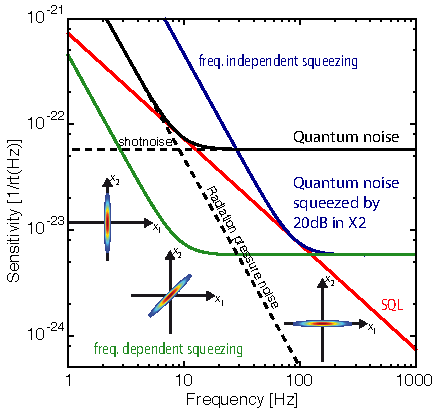
\includegraphics[width =0.5\textwidth]{./Sec_Optics/MI_SQL_AI.pdf}
\hspace{35pt}
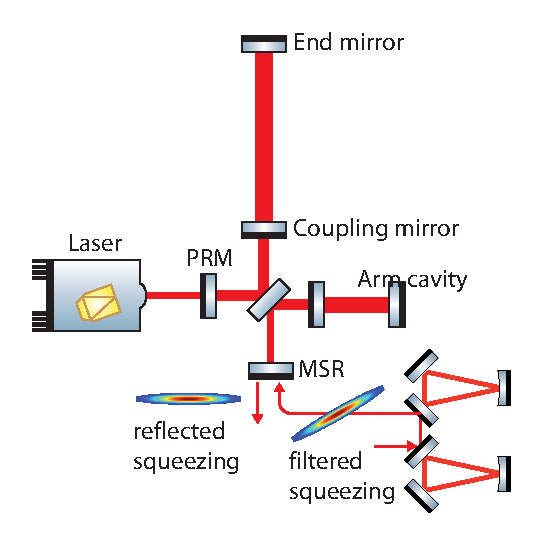
\includegraphics[scale=0.8]{./Sec_Optics/FilterMI-Ill_v2.pdf}
\caption[Illustration of frequency dependent and independent squeezed light injection]{Beating the SQL in position meter with frequency dependent light (left). Injection of frequency dependent squeezed light injection in an optical spring interferometer (right).} \label{fig:FilterMI-Ill}
\end{figure}
\subsubsection{Filter cavities}\label{sec:filtercavities}
At first view the enhancement of an interferometer's sensitivity with frequency independent squeezing (squeezed light with a fixed quadrature angle) can only be achieved in a certain frequency range. This is a direct consequence of the Heisenberg uncertainty principle. Considering a simple Michelson interferometer the quantum noise in its phase quadrature (shot noise) can be reduced by the amount of squeezing. Unfortunately, the quantum noise in the amplitude quadrature (radiation pressure noise) will be increased by the same amount enhancing the noise at low frequencies.
 
It was revealed by Unruh~\cite{Unruh1982} and others~\cite{Yuen1983, Pace1993} that squeezed field injection with frequency dependent squeezing angle allows an overall quantum noise reduction including the radiation pressure noise thereby beating the standard quantum limit (SQL). This is demonstrated in Fig.~\ref{fig:FilterMI-Ill} (left).
Figure~\ref{fig:FilterMI-Ill} (right) illustrates squeezed light injection in an optical spring interferometer. Here, an additional rotation of the squeezing ellipse is caused first by the phase-space rotation of a detuned cavity and second due to the optical spring resonance. In this case at least two filter cavities are necessary to achieve a broadband reduction of quantum noise with squeezed states of light. This is what we propose for the low-frequency ET-LF interferometer (cf. Sec.~\ref{sec:xylophone}). For the high-frequency ET-HF interferometer one filter cavity is enough (cf. Sec.~\ref{sec:xylophone} and \cite{Hild2010b}). Details about the derivation of the filter cavities design parameters are given in Appendix~\ref{app:detfcparams}.

Figure~\ref{fig:WigIll} shows the Wigner representation of a coherent vacuum state and a 20\,dB squeezed state for different squeezing angles.
\begin{figure}[H]
\centering
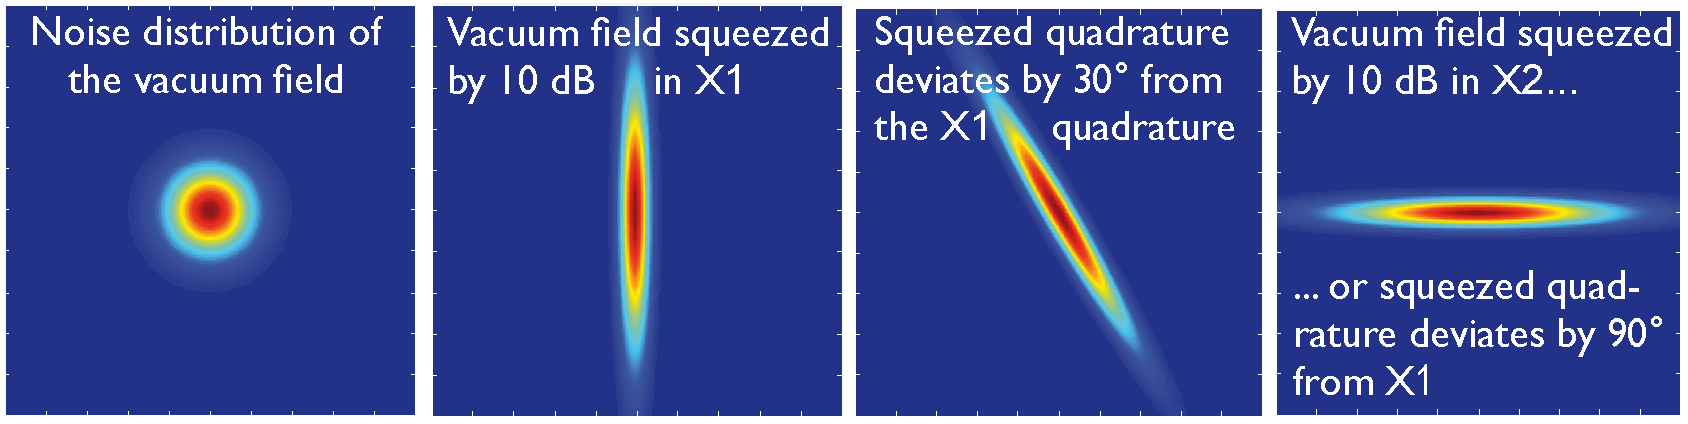
\includegraphics[width=0.7\textwidth]{Sec_Optics/WigSqzIll.pdf}%\hspace{10pt}
\caption[Wigner representation of squeezed states ]{From left to right: Wigner representation of a vacuum state (left), a pure 10\,dB amplitude squeezed state, a 10\,dB squeezed state rotated in phase-space by 30 degrees and an amplitude squeezed state rotated by 90 degrees, i.e.\ a phase squeezed state.}
\label{fig:WigIll}
\end{figure}

\FloatBarrier
\paragraph{Restrictions for the baseline length of the filter cavity}
According to the laws of quantum mechanics, whenever the optical losses (like scattering, absorbtion, etc) are encountered in the optical train, the light in the vacuum state is introduced. This generally unsqueezed light mixes up with the squeezed light thus lowering the squeezing factor of the latter. This is usually referred to as the degradation of the squeezed state which leads to the decrease of sensitivity. We demonstrate this degradation schematically in Fig.~\ref{fig:sqz-vs-loss-ill} and show dependence of the squeezing factor on the losses in Fig.~\ref{fig:sqz-vs-loss-chart}.
\begin{figure}[H]
\centering
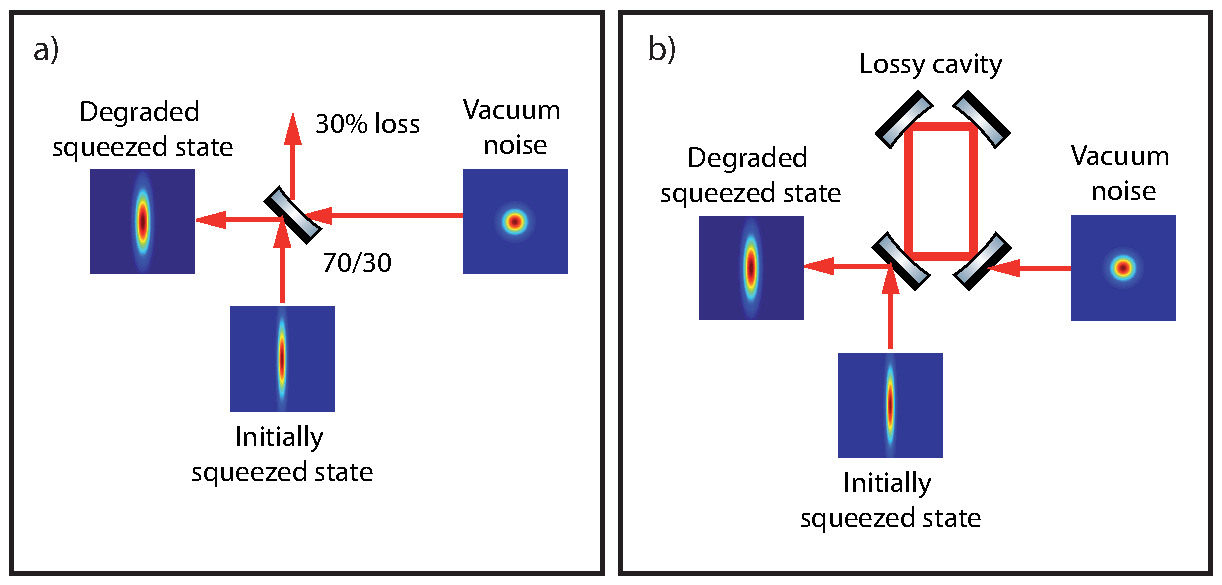
\includegraphics[scale = .6]{./Sec_Optics/Sqz-vs-loss.pdf}
\caption[Intermixture of vacuum noise to a squeezed field at lossy optics]{The figure illustrates the intermixture of vacuum noise to a squeezed field at lossy (open) ports. a) Consideration of a beam splitter  with {$R_{\rm bs} = \rho_{\rm bs}^2 = 0.7$} and {$T_{\rm bs} = \tau_{\rm bs}^2 = 0.3$}. In reflection of the beam splitter the initially squeezed state gets attenuated by the factor $\rho_{\rm bs}$. The vacuum noise couples to the reflected squeezed field with an efficiency of $\tau_{\rm bs}$ leading to a degradation of the squeezing level. b) Consideration of a lossy cavity. In this case, the intermixture of vacuum noise is frequency dependent, since the transfer function of the cavity comes into play. The degradation is maximum at the resonance frequency of the cavity. At frequencies far away from resonance the cavity behaves like an almost perfect mirror, i.e.\ the squeezing is preserved.} \label{fig:sqz-vs-loss-ill}
\end{figure}
\begin{figure}[ht]
\centering
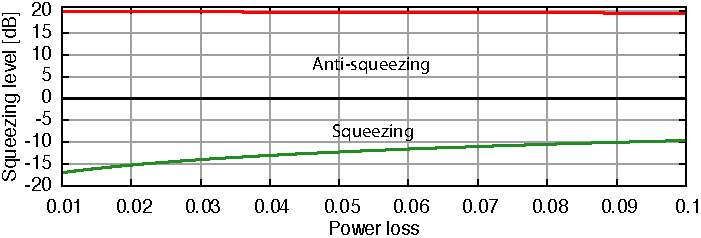
\includegraphics[scale = 1]{./Sec_Optics/SQZ-20dB-losschartAI-ill.pdf}
\caption[Degradation of a 20\,dB squeezed state due to optical loss]{The figure shows the degradation of a 20\,dB squeezed state due to optical loss. It can be seen that in contrast to the anti-squeezing level, the squeezing degrades rapidly with increasing loss. At a power loss of about 9\,\% the squeezing level is reduced from 20\,dB to 10\,dB whereas the anti-squeezing level is still about 19.6\,dB.} \label{fig:sqz-vs-loss-chart}
\end{figure}


Generally, any round-trip loss will degrade the squeezing level at
sideband frequencies being resonant in the filter cavity. For a
given power round-trip loss (mainly caused by
scattering) the resulting loss in reflection of the filter cavity
increases with a decreasing baseline length of the
filter. As well, for a certain length and a certain
round-trip loss the loss imposed on the squeezed
field increases with a decreasing half-bandwidth
that needs to be realized. The details about determination of the baseline length are given in Appendix~\ref{app:FClength}. Figure~\ref{fig:length_maintext} shows the filter cavity performance as a function of its baseline length.
\begin{figure}[ht]
\centering
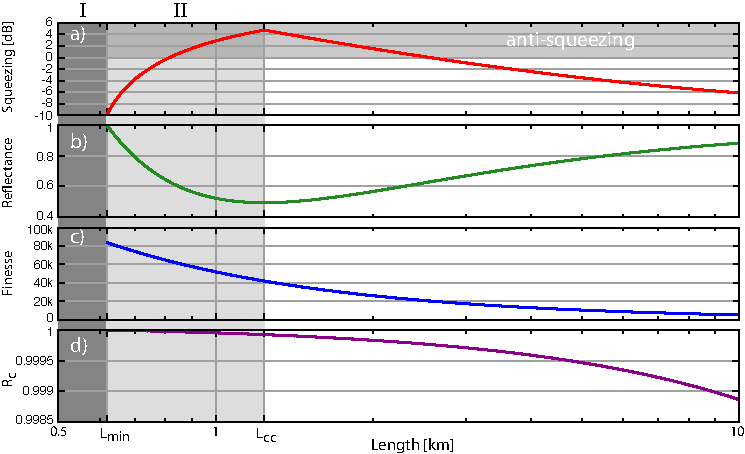
\includegraphics [scale = 1.1]{./Sec_Optics/FCslength75ppmAI.pdf}
\caption{The figure shows the filter cavity performance as a function of its baseline length $L_{\rm fc}$ (details in Appendix~\ref{app:FClength}). Graph~a) shows the remaining squeezing level in reflection of the filter cavity at its resonance frequency. Graph~b) shows the according  reflectance of the filter cavity. Graph~c) and d) show the filter cavity finesse and coupling mirror reflectance $R_{\rm c}$, respectively. The two grey shaded areas in the left highlight the region where $L_{\rm fc}<L_{\rm cc}$ (area II) and where $L_{\rm fc}<L_{\rm min}$ (area I). In the considered example ($\gamma_{\rm fc} =2\pi\cdot1.4\,{\rm Hz}$, $\Phi_{\rm fc_1}= 2\pi\cdot6.6\,{\rm Hz}\cdot L_{\rm fc_1}/c$,  $l^2_{\rm rt,fc}=75\,{\rm ppm}$) the critical length $L_{\rm cc}$ is about 1239\,m. The top grey shaded area in graph a) highlights the anti-squeezed region. Due to the unbalanced loss for upper and lower squeezing sidebands in the detuned filter cavity, for high resulting loss (i.e.\ for a cavity reflectance much smaller than one) the detected noise can be enhanced even when compared to the vacuum noise (refer to Fig.~\ref{fig:phasediffusedSQZ}). In the considered example the detected noise is already enhanced (anti-squeezed) for filter cavity baseline lengths smaller than approximately 2.5\,km.}
\label{fig:length_maintext}
\end{figure}

Our investigation demonstrated that the round-trip loss ultimately restricts the minimal allowed baseline length and consistently the performance of the filter cavities. As it is expected that the round-trip loss of the filters will be dominated by scattering at imperfect mirror surfaces, the optical layout needs to be designed such that the amount of scattering is reduced as much as possible. The scattering in different optical layouts is treated in below.
Figure~\ref{fig:sensETDHF} demonstrates the sensitivity of the ET-D-HF interferometer at various lengths of the filter cavities. Note that the high-frequency sensitivity is mostly independent of the cavity length while the low-frequency one decreases with the decrease of length.
\begin{figure}[ht]
\centering
\includegraphics{./Sec_Optics/ET-D-HF-FCs.pdf}
\caption{Sensitivity curves for ET-D-HF assuming various lengths for the filter cavity. Parameters used: round-trip loss 75ppm, 9\% frequency independent propagation loss, pure 20dB squeezing injected.}
\label{fig:sensETDHF}
\end{figure}

%%% Removed adf 27.04.2011 as the text is not complete
\begin{comment}
\longetbox{i}{box:FCdevbw}{The effect of a deviating bandwidth}{
Rotation in the wings of the FCs resonance not compensated for, thus not optimally squeezed or even enhanced noise (when compared to shot noise...
\begin{figure}[H]
\centering
\includegraphics{./Sec_Optics/FCi-devbw_reviewAI.pdf}
\caption{The figure shows the squeezing spectra for a deviation of the designed bandwidth of a) the single FC$_1$  and b) the single FC$_2$. Graph c) shows the spectra if both  filter cavities are considered. In all cases, the filter cavity round-trip loss was considered to be 75\,ppm.}
\label{fig:devBW}
\end{figure}}
\end{comment}

\paragraph{Robustness of filter cavity design parameters}
The most obvious quantities, that will potentially  change the properties of the filter are: the reflectance factors of the used mirrors, the round-trip loss, the macroscopic length, and the resonance frequency.

The first three quantities affect the bandwidth of the filter cavity and thus the required phase-space rotation around the targeted resonance frequency. A deviation from the design values of these quantities could not be compensated if the filter cavity is realised as a single resonator. An adaption of the filters bandwidth would be possible if coupled resonators---e.g.\ a linearly coupled three-mirror cavity---are utilised.  Although it should be always possible to tune the filter cavity to the required resonance frequency, for the sake of completeness we treat a potential mismatch (see details in Appendix~\ref{app:robustparam}). From the results, the requirements for the length stabilisation with regard to displacement noise could be determined. 
If a tolerable  degradation  of the squeezing  by less than 2\,dB (related to the squeezing levels  achievable with  the  design parameters) is targeted, a deviation of the bandwidth less than 5\,\% is acceptable. From this value, the tolerances for the design parameters can be deduced. 

\FloatBarrier
\begin{figure}[htb]
\centering
\includegraphics[width=0.5\textwidth]{./Sec_Optics/cavity-designs.pdf}
\caption{Four geometries were analysed from the scattering point of view.}
\label{fig:sc_geometry}
\end{figure}
\paragraph{Choosing the optical layout of the filter cavity}\label{subsec:fcscattering}

%\emph{Author(s): K. Kokeyama, A. Freise, H. L{\"u}ck}

The Einstein Telescope required two 10\,km long and one comparatively
short (several hundred meters long) filter cavities per detector. 
Such filter cavities provide the correct frequency dependence for the injected squeezing state
in order to obtain broad band quantum noise suppression in the main interferometer.
The light reflected off these cavities needs to be injected into the
interferometer dark ports. In principle any cavity geometry can 
provide the correct filtering, however, practical concerns will 
put constraints on the geometry. %In this section we briefly discuss
%these issues, while a selection of the cavity geometry has not been done at this stage.
The four cavity geometries depicted in Fig.~\ref{fig:sc_geometry} are
possible candidates;
the following advantages and disadvantages follow directly from the
geometry (given a long baseline):
\begin{itemize} 
\item the 2-mirror cavity has the advantage of using only two mirrors but
  in order to extract the reflected beam, polarising optics are
  required which introduce additional optical losses and phase noise
\item the 3-mirror cavity provides the reflected beam without the need
  for extra optics. However, the small angle between the beams at the
  far right mirror means that the setup is more sensitive to small
  angle scattering, a problem which has been seen for example in the
  triangular input mode cleaner cavity of VIRGO. Another problem is
  that the large angle of incidence on the two left mirrors requires
  the mirrors to be significant larger compared to the 2-mirror setup.
  of the 10\,km long linear arm cavities. Since the ET optical design is 
  assuming the largest available mirrors being used for the linear arm cavity, this filter
  cavity geometry can be excluded. 
\item the rectangular 4-mirror setup also has the problem of requiring
  larger mirrors due to the angle of incidence.
\item The bow-tie cavity can separate the reflected beam from the
  injected one and does not feature large angles of
  incidence so that the mirror sizes are similar to those of a linear cavity. However, it 
  is sensitive to small angle scattering.
\end{itemize}

% motivation

A detailed study of scattering in the main interferometer and the
filter cavities has not been done yet. 
In Appendix~\ref{app:scatter} we provide a first analysis of the
amount of scattering between the suspended optics itself and conclude
that this effect can be ignored in the selection of the cavity geometry. 






% memo
% mirror surface and scattering
% BRDF
% 4 topologies were compared
% you have to be careful for the rectangular cavity due to the diagonal path
% possible scattering path such as direct back scattering, the effect
% baffles
% two mirror cavity's back scattering? 
\FloatBarrier

%%% Removed adf 27.04.2011, as the text does not seem to be complete 
\begin{comment}
\paragraph{Noise couplings}\label{sec:noise}
\begin{figure}
\centering
\includegraphics[scale=0.77]{./Sec_Optics/Wig_10dB_all.jpg}
\caption{Illustration of the influence of a Gaussian distributed phase noise on the squeezed state. \textbf{Top:} Wigner functions for phase noise  with a standard deviation $\sigma$ of 0, 0.3, 0.6, 0.9. The initial, pure squeezed state was assumed with 10\,dB. \textbf{Bottom:} The probability distribution of the phase diffused squeezed states and the corresponding squeezing levels (red curves and red labels, respectively) in the  amplitude quadrature ($X_1$).  For comparison, the distribution of a vacuum state is shown (grey curves).}
\label{fig:phasediffusedSQZ}
\end{figure}

In the previous investigation comparatively high values for the phase noise was considered for illustration purpuses. Such high values are not expected to be present in a realistic experimental environment. However, the upper limit for the overall phase noise in the squeezing path depends on the squeezed state, that is generated by the squeezed light source. Table~\ref{tab:phsnoiselimit} lists the allowed phase noise (i.e.\ its standard deviation) for several conditioned squeezed states. The states were constituted for several values of the optical power  loss $l^2$ such that the  squeezing level without phase noise is 10\,dB. The required squeezing  that needs to be generated inside the squeezed light source can be calculated according to
\begin{equation}
V_s = 0.1 -l^2\hspace{11pt}\text{and}\hspace{11pt}V_a = \frac{1}{V_s}.
\end{equation}
We relates the upper limit $\sigma_{\rm max}$ for the phase noise to a squeezing level that is reduced to 9\,dB due to the phase noise. As the phase noise is assumed to be Gaussian-distributed with zero mean, Eq.~(\ref{eq:varsqzphsdiff}) can be solved giving
\begin{equation}
V_{X_1,d} = \frac{1}{2}\left[V_s+V_a+(V_s-V_a)\exp\left(-2\sigma^2\right)\right]\,.\label{eq:varianzsqzpn}
\end{equation}
Soving Eq.~(\ref{eq:varianzsqzpn}) for $\sigma$ yields
\begin{equation}
\sigma = \sqrt{-\frac{1}{2}\log\left[\frac{2V_{X_1,d}-V_s-V_a}{V_s-V_a}\right]}\,.
\end{equation}
From this equation the tolerable phase noise characterised  by $\sigma_{max}$ can be calculated for the targeted variance  $V_{X_1,d}=0.1$ and squeezing level of 10\,dB, respectively.
\begin{figure}[ht]
\centering
\includegraphics[scale=0.77]{./Sec_Optics/Wig_20dB_loss.jpg}
\caption{Degradation of a pure 20\,dB squeezed state due to optical loss and phase noise.}
\label{fig:phasediffusedSQZ20dB}
\end{figure}


\begin{table}[h]
\begin{center}
\begin{tabular}{rrrrr}
\hline
\hline
optical loss [\%]& initial squeezing [dB] & squeezing [dB] & anti-squeezing [dB] & $\sigma_{\rm max}$ \\
\hline
1 & -10.41 & -10 & 10.37 & 0.049\\
3 & -11.41 & -10 & 11.29 & 0.044\\
5 & -12.79 & -10 & 12.58 & 0.038\\
9 & -19.59 & -10 & 19.19& 0.018 \\
10 & $-\infty$ & -10 & $\infty$ & 0\\
20 & $-\infty$ & -6.99 & $\infty$ & 0\\
\hline
\hline
\end{tabular}
\end{center}
\caption{The table lists  the squeezing and anti-squeezing levels and the tolerable phase noise for several values of optical loss.}
\label{tab:phsnoiselimit}
\end{table}

From the tolerable $\sigma_{\rm max}$ we will deduce in following investigations
\begin{itemize}
\item{the allowed displacement noise in the  filter cavities}
\item{the requirements for the filter cavity length stabilization}
\item{the requirements on frequency noise of the squeezed light source related to main interferometer beam}
\end{itemize}
\FloatBarrier
\end{comment}
